\subsection{习题课 1}

\begin{exercise}
    根据如图 \ref{fig:chap1-exercise1} 所示信号 $f(t)$ 作答,其中 $t \in \set{R}$。
    \begin{enumerate}[label=(\arabic*)]
        \item 写出 $g_1(t) = f\left(\frac{t}{2}\right) * u(t)$ 的表达式,并绘出波形。
        其中,$u(t)$ 为单位阶跃函数。
        \item 绘出 $g_2(t) = f(t) * \delta(t - 2) + f(2t)$ 的波形。
    \end{enumerate}
    \begin{figure}[H]
        \centering
        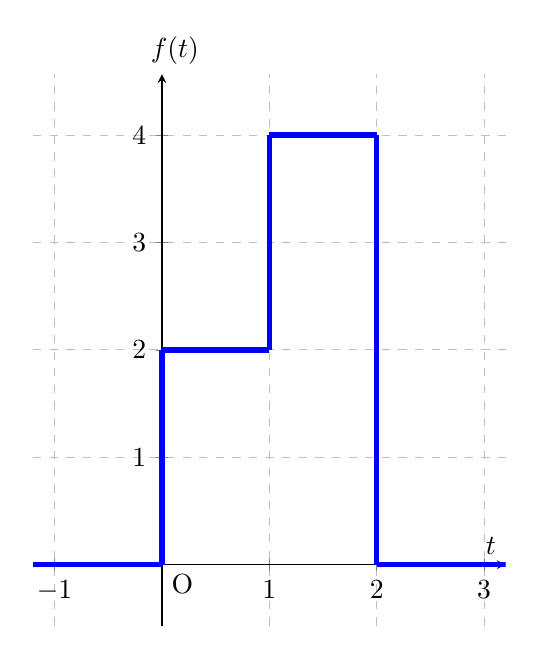
\begin{tikzpicture}
            \begin{axis}[
                axis lines = middle,
                xlabel = {$t$},
                ylabel = {$f(t)$},
                ylabel style={at={(rel axis cs:0.3, 1)}, anchor=south},
                xmin = -1.2, xmax = 3.2,
                ymin = -0.2, ymax = 4.2,
                xtick distance = 1,
                ytick distance = 1,
                grid = major,
                grid style = dashed,
                scale only axis,
                width = 6cm,
                height = 7cm,
                axis equal,
            ]
            \addplot[domain=-1.2:0, samples=100, smooth, line width=2pt, blue] {0};
            \addplot[smooth, line width=2pt, blue] coordinates {(0, 0) (0, 2)};
            \addplot[domain=0:1, samples=100, smooth, line width=2pt, blue] {2};
            \addplot[smooth, line width=2pt, blue] coordinates {(1, 2) (1, 4)};
            \addplot[domain=1:2, samples=100, smooth, line width=2pt, blue] {4};
            \addplot[smooth, line width=2pt, blue] coordinates {(2, 4) (2, 0)};
            \addplot[domain=2:3.2, samples=100, smooth, line width=2pt, blue] {0};
            \node at (axis cs:0, 0) [anchor=north west] {O};
            \end{axis}
        \end{tikzpicture}
        \caption{习题 \theexercise}
        \label{fig:chap1-exercise1}
    \end{figure}
\end{exercise}

\begin{solution}
    \begin{enumerate}[label=(\arabic*)]
        \item 由题意可得
            \begin{align*}
                g_1(t) & = f\left(\frac{t}{2}\right) * u(t) \\
                & = \int_{-\infty}^{+\infty}f\left(\frac{a}{2}\right)u(t - a)\D{a} \\
                & = \int_{-\infty}^{t}f\left(\frac{a}{2}\right)\D{a}.
            \end{align*}

            \begin{enumerate}
                \item 当 $t \le 0$ 时,$g_1(t) = \int_{-\infty}^{t}0\;\D{a} = 0$。
                \item 当 $0 < t \le 2$ 时,$g_1(t) = \int_{-\infty}^{0}0\;\D{a} + \int_{0}^{t}2\;\D{a} = 0 + 2t = 2t$。
                \item 当 $2 < t \le 4$ 时,$g_1(t) = \int_{-\infty}^{0}0\;\D{a} + \int_{0}^{2}2\;\D{a} + \int_{2}^{t}4\;\D{a} = 0 + 4 + 4(t - 2) = 4t - 4$。
                \item 当 $t > 4$ 时,$g_1(t) = \int_{-\infty}^{0}0\;\D{a} + \int_{0}^{2}2\;\D{a} + \int_{2}^{4}4\;\D{a} + \int_{4}^{t}0\;\D{a} = 0 + 4 + 8 + 0 = 12$。
            \end{enumerate}

            因此 $g_1(t)$ 的表达式为
            \begin{align*}
                g_1(t) = \begin{cases}
                    0, & t \le 0, \\
                    2t, & 0 < t \le 2, \\
                    4t - 4, & 2 < t \le 4, \\
                    12, & t > 4.
                \end{cases}
            \end{align*}

            绘制波形如图 \ref{fig:chap1-exercise1-solution1} 所示。
            \begin{figure}[H]
                \centering
                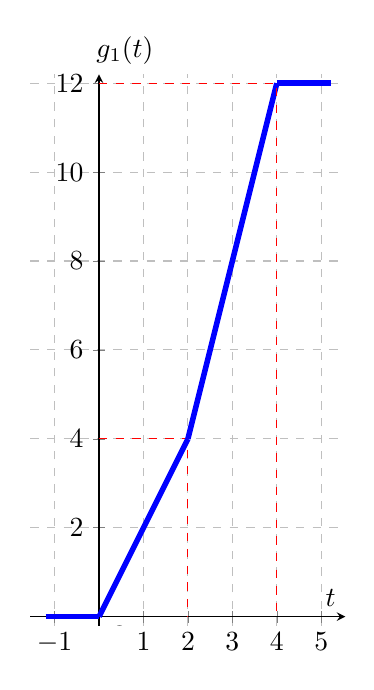
\begin{tikzpicture}
                    \begin{axis}[
                        axis lines = middle,
                        xlabel = {$t$},
                        ylabel = {$g_1(t)$},
                        ylabel style={at={(rel axis cs:0.3, 1)}, anchor=south},
                        xmin = -1.2, xmax = 5.2,
                        ymin = -0.2, ymax = 12.2,
                        xtick distance = 1,
                        ytick distance = 2,
                        grid = major,
                        grid style = dashed,
                        scale only axis,
                        width = 4cm,
                        height = 7cm,
                        axis equal,
                    ]
                    \addplot[domain=-1.2:0, samples=100, smooth, line width=2pt, blue] {0};
                    \addplot[dashed, red] coordinates {(0, 4) (2, 4) (2, 0)};
                    \addplot[domain=0:2, samples=100, smooth, line width=2pt, blue] {2 * x};
                    \addplot[domain=2:4, samples=100, smooth, line width=2pt, blue] {4 * x - 4};
                    \addplot[dashed, red] coordinates {(0, 12) (4, 12) (4, 0)};
                    \addplot[domain=4:5.2, samples=100, smooth, line width=2pt, blue] {12};
                    \node at (axis cs:0, 0) [anchor=north west] {O};
                    \end{axis}
                \end{tikzpicture}
                \caption{习题 \theexercise (1) 波形}
                \label{fig:chap1-exercise1-solution1}
            \end{figure}
        \item 由题意可得
            \begin{align*}
                g_2(t) & = f(t) * \delta(t - 2) + f(2t) \\
                & = f(t - 2) + f(2t).
            \end{align*}
            
            \begin{enumerate}
                \item 当 $t \le 0$ 时,$g_2(t) = 0 + 0 = 0$。
                \item 当 $0 < t \le \frac{1}{2}$ 时,$g_2(t) = 0 + 2 = 2$。
                \item 当 $\frac{1}{2} < t \le 1$ 时,$g_2(t) = 0 + 4 = 4$。
                \item 当 $1 < t \le 2$ 时,$g_2(t) = 0 + 0 = 0$。
                \item 当 $2 < t \le 3$ 时,$g_2(t) = 2 + 0 = 2$。
                \item 当 $3 < t \le 4$ 时,$g_2(t) = 4 + 0 = 4$。
                \item 当 $t > 4$ 时,$g_2(t) = 0 + 0 = 0$。
            \end{enumerate}

            因此 $g_2(t)$ 的表达式为
            \begin{align*}
                g_2(t) = \begin{cases}
                    0, & t \le 0, \\
                    2, & 0 < t \le \frac{1}{2}, \\
                    4, & \frac{1}{2} < t \le 1, \\
                    0, & 1 < t \le 2, \\
                    2, & 2 < t \le 3, \\
                    4, & 3 < t \le 4, \\
                    0, & t > 4.
                \end{cases}
            \end{align*}

            绘制波形如图 \ref{fig:chap1-exercise1-solution2} 所示。
            \begin{figure}[H]
                \centering
                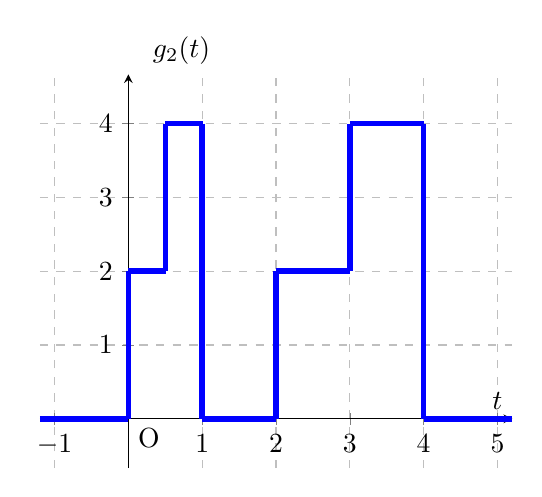
\begin{tikzpicture}
                    \begin{axis}[
                        axis lines = middle,
                        xlabel = {$t$},
                        ylabel = {$g_2(t)$},
                        ylabel style={at={(rel axis cs:0.3, 1)}, anchor=south},
                        xmin = -1.2, xmax = 5.2,
                        ymin = -0.2, ymax = 4.2,
                        xtick distance = 1,
                        ytick distance = 1,
                        grid = major,
                        grid style = dashed,
                        scale only axis,
                        width = 6cm,
                        height = 5cm,
                        axis equal,
                    ]
                    \addplot[domain=-1.2:0, samples=100, smooth, line width=2pt, blue] {0};
                    \addplot[smooth, line width=2pt, blue] coordinates {(0, 0) (0, 2)};
                    \addplot[domain=0:0.5, samples=100, smooth, line width=2pt, blue] {2};
                    \addplot[smooth, line width=2pt, blue] coordinates {(0.5, 2) (0.5, 4)};
                    \addplot[domain=0.5:1, samples=100, smooth, line width=2pt, blue] {4};
                    \addplot[smooth, line width=2pt, blue] coordinates {(1, 4) (1, 0)};
                    \addplot[domain=1:2, samples=100, smooth, line width=2pt, blue] {0};
                    \addplot[smooth, line width=2pt, blue] coordinates {(2, 0) (2, 2)};
                    \addplot[domain=2:3, samples=100, smooth, line width=2pt, blue] {2};
                    \addplot[smooth, line width=2pt, blue] coordinates {(3, 2) (3, 4)};
                    \addplot[domain=3:4, samples=100, smooth, line width=2pt, blue] {4};
                    \addplot[smooth, line width=2pt, blue] coordinates {(4, 4) (4, 0)};
                    \addplot[domain=4:5.2, samples=100, smooth, line width=2pt, blue] {0};
                    \node at (axis cs:0, 0) [anchor=north west] {O};
                    \end{axis}
                \end{tikzpicture}
                \caption{习题 \theexercise (2) 波形}
                \label{fig:chap1-exercise1-solution2}
            \end{figure}
    \end{enumerate}
\end{solution}

\begin{exercise}
    根据如图 \ref{fig:chap1-exercise2} 所示信号 $f(t)$ 作答,其中 $t \in \set{R}$。
    \begin{enumerate}[label=(\arabic*)]
        \item 写出 $g_1(t) = f(t) * \sgn{t}$ 的表达式,并绘出波形。
        \item 绘出 $g_2(t) = \sum_{n = -\infty}^{+\infty}f(t) * \delta(t - 2n)$ 的波形。
    \end{enumerate}

    \begin{figure}[H]
        \centering
        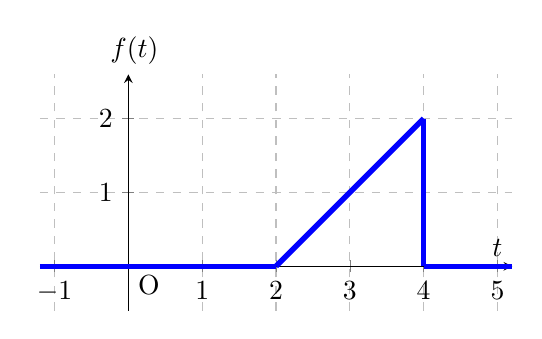
\begin{tikzpicture}
            \begin{axis}[
                axis lines = middle,
                xlabel = {$t$},
                ylabel = {$f(t)$},
                ylabel style={at={(rel axis cs:0.2, 1)}, anchor=south},
                xmin = -1.2, xmax = 5.2,
                ymin = -0.2, ymax = 2.2,
                xtick distance = 1,
                ytick distance = 1,
                grid = major,
                grid style = dashed,
                scale only axis,
                width = 6cm,
                height = 3cm,
                axis equal,
            ]
            \addplot[domain=-1.2:2, samples=100, smooth, line width=2pt, blue] {0};
            \addplot[domain=2:4, samples=100, smooth, line width=2pt, blue] {x - 2};
            \addplot[smooth, line width=2pt, blue] coordinates {(4, 2) (4, 0)};
            \addplot[domain=4:5.2, samples=100, smooth, line width=2pt, blue] {0};
            \node at (axis cs:0, 0) [anchor=north west] {O};
            \end{axis}
        \end{tikzpicture}
        \caption{习题 \theexercise}
        \label{fig:chap1-exercise2}
    \end{figure}
\end{exercise}

\begin{solution}
    \begin{enumerate}[label=(\arabic*)]
        \item 由题意可得
            \begin{align*}
                g_1(t) & = f(t) * \sgn{t} \\
                & = \int_{-\infty}^{+\infty}f(a)\sgn{t - a}\D{a} \\
                & = \int_{-\infty}^{t}f(a)\D{a} - \int_{t}^{+\infty}f(a)\D{a}.
            \end{align*}

            \begin{enumerate}
                \item 当 $t \le 2$ 时,$g_1(t)
                    = \int_{-\infty}^{t}0\;\D{a} - \left(\int_{t}^{2}0\;\D{a} + \int_{2}^{4}(a - 2)\D{a} + \int_{4}^{+\infty}0\;\D{a}\right)
                    = 0 - (0 + 2 - 0) = -2$。
                \item 当 $2 < t \le 4$ 时,$g_1(t)
                    = \left(\int_{-\infty}^{2}0\;\D{a} + \int_{2}^{t}(a - 2)\D{a}\right) - \left(\int_{t}^{4}(a - 2)\D{a} + \int_{4}^{+\infty}0\;\D{a}\right)
                    = (0 + \frac{1}{2}t^2 - 2t + 2) - (2t - \frac{1}{2}t^2 + 0)
                    = t^2 - 4t + 2$。
                \item 当 $t > 4$ 时,$g_1(t)
                    = \left(\int_{-\infty}^{2}0\;\D{a} + \int_{2}^{4}(a - 2)\D{a} + \int_{4}^{t}0\;\D{a}\right) - \left(\int_{t}^{+\infty}0\;\D{a}\right)
                    = (0 + 2 + 0) - 0
                    = 2$。
            \end{enumerate}

            因此 $g_1(t)$ 的表达式为
            \begin{align*}
                g_1(t) = \begin{cases}
                    -2, & t \le 2, \\
                    t^2 - 4t + 2, & 2 < t \le 4, \\
                    2, & t > 4.
                \end{cases}
            \end{align*}

            绘制波形如图 \ref{fig:chap1-exercise2-solution1} 所示。
            \begin{figure}[H]
                \centering
                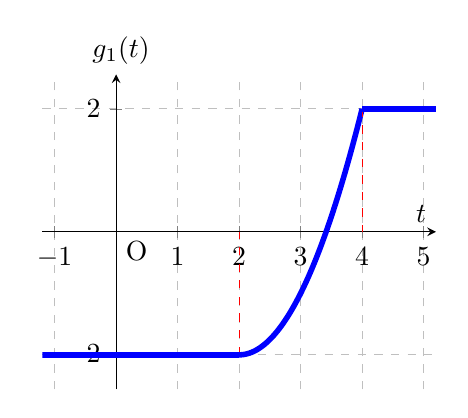
\begin{tikzpicture}
                    \begin{axis}[
                        axis lines = middle,
                        xlabel = {$t$},
                        ylabel = {$g_1(t)$},
                        ylabel style={at={(rel axis cs:0.2, 1)}, anchor=south},
                        xmin = -1.2, xmax = 5.2,
                        ymin = -2.2, ymax = 2.2,
                        xtick distance = 1,
                        ytick distance = 2,
                        grid = major,
                        grid style = dashed,
                        scale only axis,
                        width = 5cm,
                        height = 4cm,
                        axis equal,
                    ]
                    \addplot[domain=-1.2:2, samples=100, smooth, line width=2pt, blue] {-2};
                    \addplot[dashed, red] coordinates {(2, -2) (2, 0)};
                    \addplot[domain=2:4, samples=100, smooth, line width=2pt, blue] {x * x - 4 * x + 2};
                    \addplot[dashed, red] coordinates {(4, 2) (4, 0)};
                    \addplot[domain=4:5.2, samples=100, smooth, line width=2pt, blue] {2};
                    \node at (axis cs:0, 0) [anchor=north west] {O};
                    \end{axis}
                \end{tikzpicture}
                \caption{习题 \theexercise (1) 波形}
                \label{fig:chap1-exercise2-solution1}
            \end{figure}
        \item 由题意可得 $g_2(t) = \sum_{n = -\infty}^{+\infty}f(t - 2n)$,
            这等价于将 $f(t)$ 沿 $t$ 轴左右平移偶数格后叠加。
            因此 $g_2(t)$ 为周期函数,波形图如图 \ref{fig:chap1-exercise2-solution2} 所示。
            \begin{figure}[H]
                \centering
                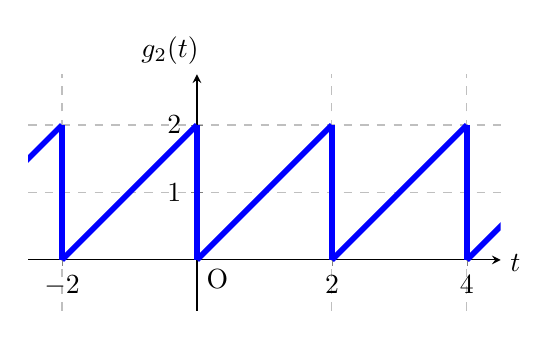
\begin{tikzpicture}
                    \begin{axis}[
                        axis lines = middle,
                        xlabel = {$t$},
                        xlabel style={at={(rel axis cs:1, 0.2)}, anchor=west},
                        ylabel = {$g_2(t)$},
                        ylabel style={at={(rel axis cs:0.3, 1)}, anchor=south},
                        xmin = -2.5, xmax = 4.5,
                        ymin = -0.2, ymax = 2.2,
                        xtick distance = 2,
                        ytick distance = 1,
                        grid = major,
                        grid style = dashed,
                        scale only axis,
                        width = 6cm,
                        height = 3cm,
                        axis equal,
                    ]
                    \addplot[domain=-3:-2, samples=100, smooth, line width=2pt, blue] {x + 4};
                    \addplot[smooth, line width=2pt, blue] coordinates {(-2, 2) (-2, 0)};
                    \addplot[domain=-2:0, samples=100, smooth, line width=2pt, blue] {x + 2};
                    \addplot[smooth, line width=2pt, blue] coordinates {(0, 2) (0, 0)};
                    \addplot[domain=0:2, samples=100, smooth, line width=2pt, blue] {x};
                    \addplot[smooth, line width=2pt, blue] coordinates {(2, 2) (2, 0)};
                    \addplot[domain=2:4, samples=100, smooth, line width=2pt, blue] {x - 2};
                    \addplot[smooth, line width=2pt, blue] coordinates {(4, 2) (4, 0)};
                    \addplot[domain=4:5, samples=100, smooth, line width=2pt, blue] {x - 4};
                    \node at (axis cs:0, 0) [anchor=north west] {O};
                    \end{axis}
                \end{tikzpicture}
                \caption{习题 \theexercise (2) 波形}
                \label{fig:chap1-exercise2-solution2}
            \end{figure}
    \end{enumerate}
\end{solution}

\begin{exercise}
    根据如图 \ref{fig:chap1-exercise3} 所示信号 $f(t)$ 作答,其中 $t \in \set{R}$。
    \begin{enumerate}[label=(\arabic*)]
        \item 写出 $g_1(t) = f(t) * G_1(t)$ 的表达式,并绘出波形。
            其中,$G_1(t)$ 为脉高和脉宽均为 $1$ 的矩形脉冲信号。
        \item 绘出 $g_2(t) = \sum_{n = -\infty}^{+\infty}f(t) * \delta(t - 2n)$ 的波形。
    \end{enumerate}

    \begin{figure}[H]
        \centering
        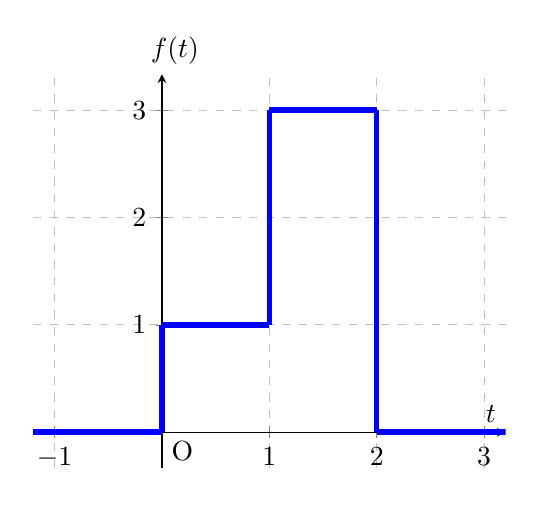
\begin{tikzpicture}
            \begin{axis}[
                axis lines = middle,
                xlabel = {$t$},
                ylabel = {$f(t)$},
                ylabel style={at={(rel axis cs:0.3, 1)}, anchor=south},
                xmin = -1.2, xmax = 3.2,
                ymin = -0.2, ymax = 3.2,
                xtick distance = 1,
                ytick distance = 1,
                grid = major,
                grid style = dashed,
                scale only axis,
                width = 6cm,
                height = 5cm,
                axis equal,
            ]
            \addplot[domain=-1.2:0, samples=100, smooth, line width=2pt, blue] {0};
            \addplot[smooth, line width=2pt, blue] coordinates {(0, 0) (0, 1)};
            \addplot[domain=0:1, samples=100, smooth, line width=2pt, blue] {1};
            \addplot[smooth, line width=2pt, blue] coordinates {(1, 1) (1, 3)};
            \addplot[domain=1:2, samples=100, smooth, line width=2pt, blue] {3};
            \addplot[smooth, line width=2pt, blue] coordinates {(2, 3) (2, 0)};
            \addplot[domain=2:3.2, samples=100, smooth, line width=2pt, blue] {0};
            \node at (axis cs:0, 0) [anchor=north west] {O};
            \end{axis}
        \end{tikzpicture}
        \caption{习题 \theexercise}
        \label{fig:chap1-exercise3}
    \end{figure}
\end{exercise}

\begin{solution}
    \begin{enumerate}[label=(\arabic*)]
        \item 由题意可得
            \begin{align*}
                g_1(t) & = f(t) * G_1(t) \\
                & = \int_{-\infty}^{+\infty}f(a)G_1(t - a)\D{a} \\
                & = \int_{t - 1/2}^{t + 1/2}f(a)\D{a}
            \end{align*}

            \begin{enumerate}
                \item 当 $t \le -\frac{1}{2}$ 时,$g_1(t) = \int_{t - 1/2}^{t + 1/2}0\;\D{a} = 0$。
                \item 当 $-\frac{1}{2} < t \le \frac{1}{2}$ 时,$g_1(t)
                    = \int_{t - 1/2}^{0}0\;\D{a} + \int_{0}^{t + 1/2}1\;\D{a}
                    = t + \frac{1}{2}$。
                \item 当 $\frac{1}{2} < t \le \frac{3}{2}$ 时,$g_1(t)
                    = \int_{t - 1/2}^{1}1\;\D{a} + \int_{1}^{t + 1/2}3\;\D{a}
                    = 2t$。
                \item 当 $\frac{3}{2} < t \le \frac{5}{2}$ 时,$g_1(t)
                    = \int_{t - 1/2}^{2}3\;\D{a} + \int_{2}^{t + 1/2}0\;\D{a}
                    = \frac{15}{2} - 3t$。
                \item 当 $t > \frac{5}{2}$ 时,$g_1(t) = \int_{t - 1/2}^{t + 1/2}0\;\D{a} = 0$。
            \end{enumerate}

            因此 $g_1(t)$ 的表达式为
            \begin{align*}
                g_1(t) = \begin{cases}
                    0, & t \le -\frac{1}{2}, \\
                    t + \frac{1}{2}, & -\frac{1}{2} < t \le \frac{1}{2}, \\
                    2t, & \frac{1}{2} < t \le \frac{3}{2}, \\
                    \frac{15}{2} - 3t, & \frac{3}{2} < t \le \frac{5}{2}, \\
                    0, & t > \frac{5}{2}.
                \end{cases}
            \end{align*}

            绘制波形如图 \ref{fig:chap1-exercise3-solution1} 所示。
            \begin{figure}[H]
                \centering
                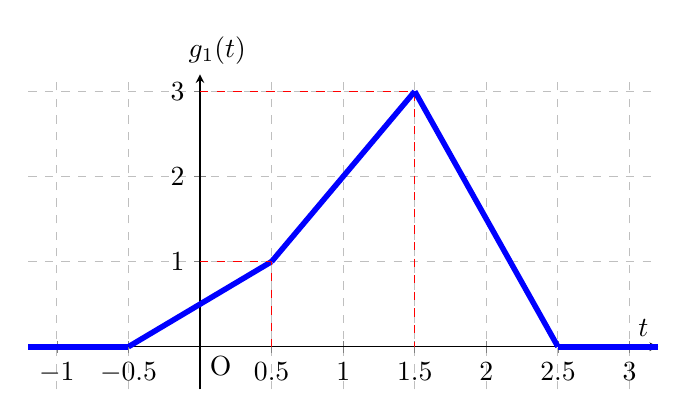
\begin{tikzpicture}
                    \begin{axis}[
                        axis lines = middle,
                        xlabel = {$t$},
                        ylabel = {$g_1(t)$},
                        ylabel style={at={(rel axis cs:0.3, 1)}, anchor=south},
                        xmin = -1.2, xmax = 3.2,
                        ymin = -0.5, ymax = 3.2,
                        xtick distance = 0.5,
                        ytick distance = 1,
                        grid = major,
                        grid style = dashed,
                        scale only axis,
                        width = 8cm,
                        height = 4cm,
                    ]
                    \addplot[domain=-1.2:-0.5, samples=100, smooth, line width=2pt, blue] {0};
                    \addplot[domain=-0.5:0.5, samples=100, smooth, line width=2pt, blue] {x + 0.5};
                    \addplot[dashed, red] coordinates {(0, 1) (0.5, 1) (0.5, 0)};
                    \addplot[domain=0.5:1.5, samples=100, smooth, line width=2pt, blue] {2 * x};
                    \addplot[dashed, red] coordinates {(0, 3) (1.5, 3) (1.5, 0)};
                    \addplot[domain=1.5:2.5, samples=100, smooth, line width=2pt, blue] {15 / 2 - 3 * x};
                    \addplot[domain=2.5:3.2, samples=100, smooth, line width=2pt, blue] {0};
                    \node at (axis cs:0, 0) [anchor=north west] {O};
                    \end{axis}
                \end{tikzpicture}
                \caption{习题 \theexercise (1) 波形}
                \label{fig:chap1-exercise3-solution1}
            \end{figure}
        \item 由题意可得 $g_2(t) = \sum_{n = -\infty}^{+\infty}f(t - 2n)$,
            这等价于将 $f(t)$ 沿 $t$ 轴左右平移偶数格后叠加。
            因此 $g_2(t)$ 为周期函数,波形图如图 \ref{fig:chap1-exercise3-solution2} 所示。
            \begin{figure}[H]
                \centering
                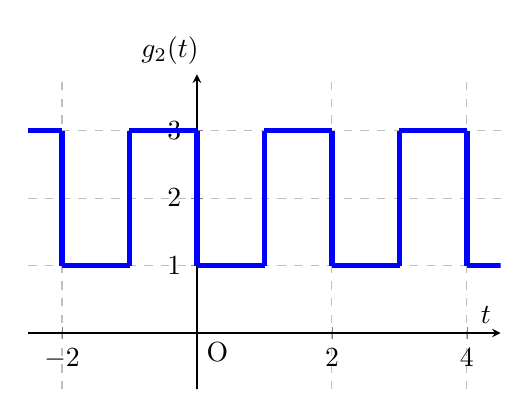
\begin{tikzpicture}
                    \begin{axis}[
                        axis lines = middle,
                        xlabel = {$t$},
                        ylabel = {$g_2(t)$},
                        ylabel style={at={(rel axis cs:0.3, 1)}, anchor=south},
                        xmin = -2.5, xmax = 4.5,
                        ymin = -0.2, ymax = 3.2,
                        xtick distance = 2,
                        ytick distance = 1,
                        grid = major,
                        grid style = dashed,
                        scale only axis,
                        width = 6cm,
                        height = 4cm,
                        axis equal,
                    ]
                    \addplot[domain=-3:-2, samples=100, smooth, line width=2pt, blue] {3};
                    \addplot[smooth, line width=2pt, blue] coordinates {(-2, 3) (-2, 1)};
                    \addplot[domain=-2:-1, samples=100, smooth, line width=2pt, blue] {1};
                    \addplot[smooth, line width=2pt, blue] coordinates {(-1, 1) (-1, 3)};
                    \addplot[domain=-1:0, samples=100, smooth, line width=2pt, blue] {3};
                    \addplot[smooth, line width=2pt, blue] coordinates {(0, 3) (0, 1)};
                    \addplot[domain=0:1, samples=100, smooth, line width=2pt, blue] {1};
                    \addplot[smooth, line width=2pt, blue] coordinates {(1, 1) (1, 3)};
                    \addplot[domain=1:2, samples=100, smooth, line width=2pt, blue] {3};
                    \addplot[smooth, line width=2pt, blue] coordinates {(2, 3) (2, 1)};
                    \addplot[domain=2:3, samples=100, smooth, line width=2pt, blue] {1};
                    \addplot[smooth, line width=2pt, blue] coordinates {(3, 1) (3, 3)};
                    \addplot[domain=3:4, samples=100, smooth, line width=2pt, blue] {3};
                    \addplot[smooth, line width=2pt, blue] coordinates {(4, 3) (4, 1)};
                    \addplot[domain=4:5, samples=100, smooth, line width=2pt, blue] {1};
                    \node at (axis cs:0, 0) [anchor=north west] {O};
                    \end{axis}
                \end{tikzpicture}
                \caption{习题 \theexercise (2) 波形}
                \label{fig:chap1-exercise3-solution2}
            \end{figure}
    \end{enumerate}
\end{solution}

\begin{exercise}
    根据如图 \ref{fig:chap1-exercise4} 所示信号 $f(t)$ 作答,其中 $t \in \set{R}$。
    \begin{enumerate}[label=(\arabic*)]
        \item 绘出 $g_1(t) = \sum_{n = -\infty}^{+\infty}f(t) * \delta(t - 2n)$ 的波形。
        \item 绘出 $g_2(t) = f(t) * f(t)$ 的波形。
    \end{enumerate}

    \begin{figure}[H]
        \centering
        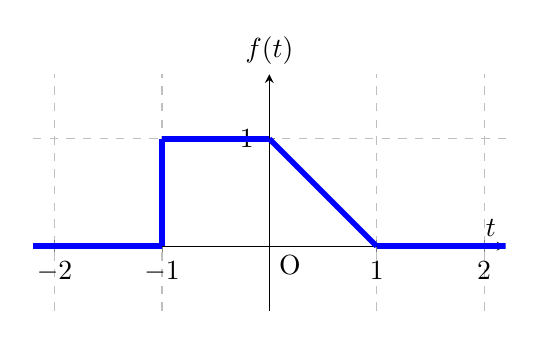
\begin{tikzpicture}
            \begin{axis}[
                axis lines = middle,
                xlabel = {$t$},
                ylabel = {$f(t)$},
                ylabel style={at={(rel axis cs:0.5, 1)}, anchor=south},
                xmin = -2.2, xmax = 2.2,
                ymin = -0.2, ymax = 1.2,
                xtick distance = 1,
                ytick distance = 1,
                grid = major,
                grid style = dashed,
                scale only axis,
                width = 6cm,
                height = 3cm,
                axis equal,
            ]
            \addplot[domain=-2.2:-1, samples=100, smooth, line width=2pt, blue] {0};
            \addplot[smooth, line width=2pt, blue] coordinates {(-1, 0) (-1, 1)};
            \addplot[domain=-1:0, samples=100, smooth, line width=2pt, blue] {1};
            \addplot[domain=0:1, samples=100, smooth, line width=2pt, blue] {1 - x};
            \addplot[domain=1:2.2, samples=100, smooth, line width=2pt, blue] {0};
            \node at (axis cs:0, 0) [anchor=north west] {O};
            \end{axis}
        \end{tikzpicture}
        \caption{习题 \theexercise}
        \label{fig:chap1-exercise4}
    \end{figure}
\end{exercise}

\begin{solution}
    \begin{enumerate}[label=(\arabic*)]
        \item 由题意可得 $g_1(t) = \sum_{n = -\infty}^{+\infty}f(t - 2n)$,
            这等价于将 $f(t)$ 沿 $t$ 轴左右平移偶数格后叠加。
            因此 $g_1(t)$ 为周期函数,波形图如图 \ref{fig:chap1-exercise4-solution1} 所示。
            \begin{figure}[H]
                \centering
                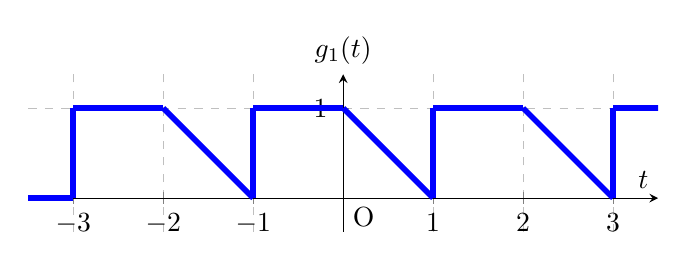
\begin{tikzpicture}
                    \begin{axis}[
                        axis lines = middle,
                        xlabel = {$t$},
                        ylabel = {$g_1(t)$},
                        ylabel style={at={(rel axis cs:0.5, 1)}, anchor=south},
                        xmin = -3.5, xmax = 3.5,
                        ymin = -0.2, ymax = 1.2,
                        xtick distance = 1,
                        ytick distance = 1,
                        grid = major,
                        grid style = dashed,
                        scale only axis,
                        width = 8cm,
                        height = 2cm,
                        axis equal,
                    ]
                    \addplot[domain=-4:-3, samples=100, smooth, line width=2pt, blue] {0};
                    \addplot[smooth, line width=2pt, blue] coordinates {(-3, 0) (-3, 1)};
                    \addplot[domain=-3:-2, samples=100, smooth, line width=2pt, blue] {1};
                    \addplot[domain=-2:-1, samples, smooth, line width=2pt, blue] {-x - 1};
                    \addplot[smooth, line width=2pt, blue] coordinates {(-1, 0) (-1, 1)};
                    \addplot[domain=-1:0, samples=100, smooth, line width=2pt, blue] {1};
                    \addplot[domain=0:1, samples=100, smooth, line width=2pt, blue] {-x + 1};
                    \addplot[smooth, line width=2pt, blue] coordinates {(1, 0) (1, 1)};
                    \addplot[domain=1:2, samples=100, smooth, line width=2pt, blue] {1};
                    \addplot[domain=2:3, samples=100, smooth, line width=2pt, blue] {-x + 3};
                    \addplot[smooth, line width=2pt, blue] coordinates {(3, 0) (3, 1)};
                    \addplot[domain=3:4, samples=100, smooth, line width=2pt, blue] {1};
                    \node at (axis cs:0, 0) [anchor=north west] {O};
                    \end{axis}
                \end{tikzpicture}
                \caption{习题 \theexercise (1) 波形}
                \label{fig:chap1-exercise4-solution1}
            \end{figure}
        \item 由题意可得
            \begin{align*}
                g_2(t) & = f(t) * f(t) \\
                & = \int_{-\infty}^{+\infty}f(a)f(t - a)\D{a} \\
                & = \int_{t - 1}^{t}(1 - t + a)f(a)\D{a} + \int_{t}^{t + 1}f(a)\D{a}.
            \end{align*}

            \begin{enumerate}
                \item 当 $t \le -2$ 时,有
                    \begin{align*}
                        g_2(t) & = \int_{t - 1}^{t}(1 - t + a) \cdot 0\;\D{a} + \int_{t}^{t + 1}0\;\D{a} \\
                        & = 0.
                    \end{align*}
                \item 当 $-2 < t \le -1$ 时,有
                    \begin{align*}
                        g_2(t) & = \int_{t - 1}^{t}(1 - t + a) \cdot 0\;\D{a} + \int_{t}^{-1}0\;\D{a} + \int_{-1}^{t + 1}1\;\D{a} \\
                        & = 0 + 0 + t + 2 \\
                        & = t + 2.
                    \end{align*}
                \item 当 $-1 < t \le 0$ 时,有
                    \begin{align*}
                        g_2(t) & = \int_{t - 1}^{-1}(1 - t + a)\cdot 0\;\D{a} + \int_{-1}^{t}(1 - t + a)\cdot 1\;\D{a} + \int_{t}^{0}1\;\D{a} + \int_{0}^{t + 1}(1 - a)\D{a} \\
                        & = \left.0 + \left.\left(\frac{1}{2}a^2 + (1 - t)a\right)\right|_{a = -1}^{a = t} - t + \left(-\frac{1}{2}a^2 + a\right)\right|_{a = 0}^{a = t + 1} \\
                        & = \left(-\frac{1}{2}t^2 + t\right) - \left(t - \frac{1}{2}\right) - t + \left(-\frac{1}{2}t^2 + \frac{1}{2}\right) \\
                        & = -t^2 - t + 1.
                    \end{align*}
                \item 当 $0 < t \le 1$ 时,有
                    \begin{align*}
                        g_2(t) & = \int_{t - 1}^{0}(1 - t + a)\cdot 1\;\D{a} + \int_{0}^{t}(1 - t + a)(1 - a)\D{a} + \int_{t}^{1}(1 - a)\D{a} + \int_{1}^{t + 1}0\;\D{a} \\
                        & = \int_{t - 1}^{0}(1 - t + a)\D{a} + \int_{0}^{t}(-a^2 + ta - (t - 1))\D{a} + \int_{t}^{1}(1 - a)\D{a} + 0 \\
                        & = \left.\left(\frac{1}{2}a^2 + (1 - t)a\right)\right|_{a = t - 1}^{a = 0} + \left.\left(-\frac{1}{3}a^3 + \frac{1}{2}ta^2 - (t - 1)a\right)\right|_{a = 0}^{a = t} + \left.\left(-\frac{1}{2}a^2 + a\right)\right|_{a = t}^{a = 1} \\
                        & = 0 - \left(-\frac{1}{2}t^2 + t - \frac{1}{2}\right) + \left(\frac{1}{6}t^3 - t^2 + t\right) + \frac{1}{2} - \left(-\frac{1}{2}t^2 + t\right) \\
                        & = \frac{1}{6}t^3 - t + 1.
                    \end{align*}
                \item 当 $1 < t \le 2$ 时,有
                    \begin{align*}
                        g_2(t) & = \int_{t - 1}^{1}(1 - t + a)(1 - a)\D{a} + \int_{1}^{t}(1 - t + a)\cdot 0\;\D{a} + \int_{t}^{t + 1}0\;\D{a} \\
                        & = \int_{t - 1}^{1}(-a^2 + ta - (t - 1))\D{a} + 0 + 0 \\
                        & = \left.\left(-\frac{1}{3}a^3 + \frac{1}{2}ta^2 - (t - 1)a\right)\right|_{a = t - 1}^{a = 1} \\
                        & = \left(-\frac{1}{2}t + \frac{2}{3}\right) - \left(\frac{1}{6}t^3 - t^2 + \frac{3}{2}t - \frac{2}{3}\right) \\
                        & = -\frac{1}{6}t^3 + t^2 - 2t + \frac{4}{3}.
                    \end{align*}
                \item 当 $t > 2$ 时,有
                    \begin{align*}
                        g_2(t) & = \int_{t - 1}^{t}(1 - t + 1) \cdot 0\;\D{a} + \int_{t}^{t + 1}0\;\D{a} \\
                        & = 0.
                    \end{align*}
            \end{enumerate}

            因此 $g_2(t)$ 的表达式为
            \begin{align*}
                g_2(t) = \begin{cases}
                    0, & t \le -2, \\
                    t + 2, & -2 < t \le -1, \\
                    -t^2 - t + 1, & -1 < t \le 0, \\
                    \frac{1}{6}t^3 - t + 1, & 0 < t \le 1, \\
                    -\frac{1}{6}t^3 + t^2 - 2t + \frac{4}{3}, & 1 < t \le 2, \\
                    0, & t > 2.
                \end{cases}
            \end{align*}

            绘制波形如图 \ref{fig:chap1-exercise4-solution2} 所示。
            \begin{figure}[H]
                \centering
                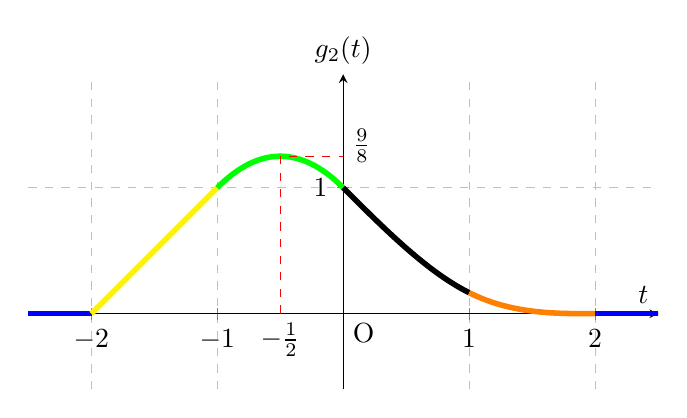
\begin{tikzpicture}
                    \begin{axis}[
                        axis lines = middle,
                        xlabel = {$t$},
                        ylabel = {$g_2(t)$},
                        ylabel style={at={(rel axis cs:0.5, 1)}, anchor=south},
                        xmin = -2.5, xmax = 2.5,
                        ymin = -0.2, ymax = 1.5,
                        xtick distance = 1,
                        ytick distance = 1,
                        grid = major,
                        grid style = dashed,
                        scale only axis,
                        width = 8cm,
                        height = 4cm,
                        axis equal,
                    ]
                    \addplot[domain=-2.5:-2, samples=100, smooth, line width=2pt, blue] {0};
                    \addplot[domain=-2:-1, samples=100, smooth, line width=2pt, yellow] {x + 2};
                    \addplot[domain=-1:0, samples=100, smooth, line width=2pt, green] {-x * x - x + 1};
                    \addplot[dashed, red] coordinates {(-0.5, 0) (-0.5, 1.25) (0, 1.25)};
                    \node at (axis cs:-0.5, 0) [anchor=north] {$-\frac{1}{2}$};
                    \node at (axis cs:0, 1.125) [anchor=south west] {$\frac{9}{8}$};
                    \addplot[domain=0:1, samples=100, smooth, line width=2pt, black] {x * x * x / 6 - x + 1};
                    \addplot[domain=1:2, samples=100, smooth, line width=2pt, orange] {-x * x * x / 6 + x * x - 2 * x + 4 / 3};
                    \addplot[domain=2:2.5, samples=100, smooth, line width=2pt, blue] {0};
                    \node at (axis cs:0, 0) [anchor=north west] {O};
                    \end{axis}
                \end{tikzpicture}
                \caption{习题 \theexercise (2) 波形}
                \label{fig:chap1-exercise4-solution2}
            \end{figure}
    \end{enumerate}
\end{solution}

\begin{exercise}
    根据如图 \ref{fig:chap1-exercise5} 所示信号 $f(t)$ 作答,其中 $t \in \set{R}$。
    \begin{enumerate}[label=(\arabic*)]
        \item 绘出 $g_1(t) = \sum_{n = -\infty}^{+\infty}f(t + 1) * \delta(t - 2n)$ 的波形。
        \item 绘出 $g_2(t) = f(2t) * \sgn{t + 1}$ 的波形。
    \end{enumerate}

    \begin{figure}[H]
        \centering
        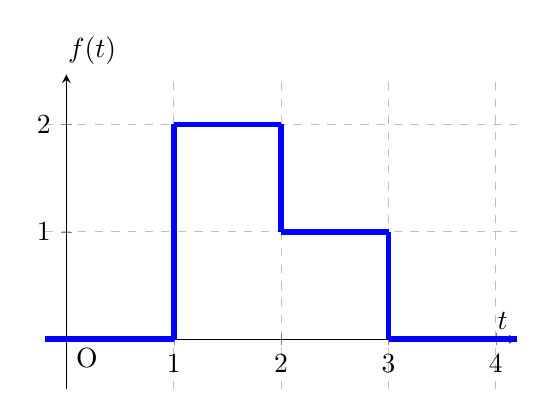
\begin{tikzpicture}
            \begin{axis}[
                axis lines = middle,
                xlabel = {$t$},
                ylabel = {$f(t)$},
                ylabel style={at={(rel axis cs:0.1, 1)}, anchor=south},
                xmin = -0.2, xmax = 4.2,
                ymin = -0.2, ymax = 2.2,
                xtick distance = 1,
                ytick distance = 1,
                grid = major,
                grid style = dashed,
                scale only axis,
                width = 6cm,
                height = 4cm,
                axis equal,
            ]
            \addplot[domain=-0.2:1, samples=100, smooth, line width=2pt, blue] {0};
            \addplot[smooth, line width=2pt, blue] coordinates {(1, 0) (1, 2)};
            \addplot[domain=1:2, samples=100, smooth, line width=2pt, blue] {2};
            \addplot[smooth, line width=2pt, blue] coordinates {(2, 2) (2, 1)};
            \addplot[domain=2:3, samples=100, smooth, line width=2pt, blue] {1};
            \addplot[smooth, line width=2pt, blue] coordinates {(3, 1) (3, 0)};
            \addplot[domain=3:4.2, samples=100, smooth, line width=2pt, blue] {0};
            \node at (axis cs:0, 0) [anchor=north west] {O};
            \end{axis}
        \end{tikzpicture}
        \caption{习题 \theexercise}
        \label{fig:chap1-exercise5}
    \end{figure}
\end{exercise}

\begin{solution}
    \begin{enumerate}[label=(\arabic*)]
        \item 由题意可得 $g_1(t) = \sum_{n = -\infty}^{+\infty}f(t + 1 - 2n)$,
            这等价于将 $f(t)$ 沿 $t$ 轴左右平移奇数格后叠加。
            因此 $g_1(t)$ 为周期函数,波形图如图 \ref{fig:chap1-exercise5-solution1} 所示。
            \begin{figure}[H]
                \centering
                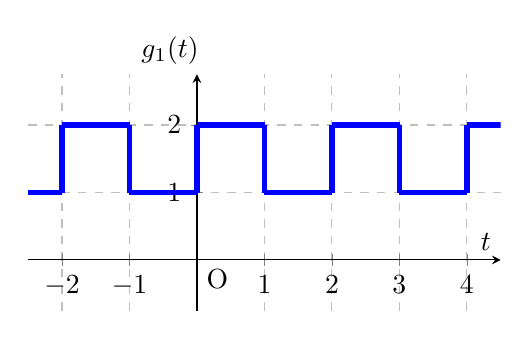
\begin{tikzpicture}
                    \begin{axis}[
                        axis lines = middle,
                        xlabel = {$t$},
                        ylabel = {$g_1(t)$},
                        ylabel style={at={(rel axis cs:0.3, 1)}, anchor=south},
                        xmin = -2.5, xmax = 4.5,
                        ymin = -0.2, ymax = 2.2,
                        xtick distance = 1,
                        ytick distance = 1,
                        grid = major,
                        grid style = dashed,
                        scale only axis,
                        width = 6cm,
                        height = 3cm,
                        axis equal,
                    ]
                    \addplot[domain=-3:-2, samples=100, smooth, line width=2pt, blue] {1};
                    \addplot[smooth, line width=2pt, blue] coordinates {(-2, 1) (-2, 2)};
                    \addplot[domain=-2:-1, samples=100, smooth, line width=2pt, blue] {2};
                    \addplot[smooth, line width=2pt, blue] coordinates {(-1, 2) (-1, 1)};
                    \addplot[domain=-1:0, samples=100, smooth, line width=2pt, blue] {1};
                    \addplot[smooth, line width=2pt, blue] coordinates {(0, 1) (0, 2)};
                    \addplot[domain=0:1, samples=100, smooth, line width=2pt, blue] {2};
                    \addplot[smooth, line width=2pt, blue] coordinates {(1, 2) (1, 1)};
                    \addplot[domain=1:2, samples=100, smooth, line width=2pt, blue] {1};
                    \addplot[smooth, line width=2pt, blue] coordinates {(2, 1) (2, 2)};
                    \addplot[domain=2:3, samples=100, smooth, line width=2pt, blue] {2};
                    \addplot[smooth, line width=2pt, blue] coordinates {(3, 2) (3, 1)};
                    \addplot[domain=3:4, samples=100, smooth, line width=2pt, blue] {1};
                    \addplot[smooth, line width=2pt, blue] coordinates {(4, 1) (4, 2)};
                    \addplot[domain=4:5, samples=100, smooth, line width=2pt, blue] {2};
                    \node at (axis cs:0, 0) [anchor=north west] {O};
                    \end{axis}
                \end{tikzpicture}
                \caption{习题 \theexercise (1) 波形}
                \label{fig:chap1-exercise5-solution1}
            \end{figure}
        \item 由题意可得
            \begin{align*}
                g_2(t) & = f(2t) * \sgn{t + 1} \\
                & = \int_{-\infty}^{+\infty}f(2a)\sgn{t - a + 1}\D{a} \\
                & = \int_{-\infty}^{t - 1}f(2a)\D{a} - \int_{t - 1}^{+\infty}f(2a)\D{a}.
            \end{align*}

            \begin{enumerate}
                \item 当 $t \le -\frac{1}{2}$ 时,$g_2(t)
                    = \int_{-\infty}^{t + 1}0\;\D{a} - \left(\int_{t + 1}^{1/2}0\;\D{a} + \int_{1/2}^{1}2\;\D{a} + \int_{1}^{3/2}1\;\D{a} + \int_{3/2}^{+\infty}0\;\D{a}\right)
                    = 0 - (0 + 1 + \frac{1}{2} + 0)
                    = -\frac{3}{2}$。
                \item 当 $-\frac{1}{2} < t \le 0$ 时,$g_2(t)
                    = \left(\int_{-\infty}^{1/2}0\;\D{a} + \int_{1/2}^{t + 1}2\;\D{a}\right) - \left(\int_{t + 1}^{1}2\;\D{a} + \int_{1}^{3/2}1\;\D{a} + \int_{3/2}^{+\infty}0\;\D{a}\right)
                    = (0 + 2t + 1) - (-2t + \frac{1}{2} + 0)
                    = 4t + \frac{1}{2}$。
                \item 当 $0 < t \le \frac{1}{2}$ 时,$g_2(t)
                    = \left(\int_{-\infty}^{1/2}0\;\D{a} + \int_{1/2}^{1}2\;\D{a} + \int_{1}^{t + 1}1\;\D{a}\right) - \left(\int_{t + 1}^{3/2}1\;\D{a} + \int_{3/2}^{+\infty}0\;\D{a}\right)
                    = (0 + 1 + t) - (\frac{1}{2} - t + 0)
                    = 2t + \frac{1}{2}$。
                \item 当 $t > \frac{1}{2}$ 时,$g_2(t)
                    = \left(\int_{-\infty}^{1/2}0\;\D{a} + \int_{1/2}^{1}2\;\D{a} + \int_{1}^{3/2}1\;\D{a} + \int_{3/2}^{t + 1}0\;\D{a}\right) - \int_{t + 1}^{+\infty}0\;\D{a}
                    = (0 + 1 + \frac{1}{2} + 0) - 0
                    = \frac{3}{2}$。
            \end{enumerate}

            因此 $g_2(t)$ 的表达式为
            \begin{align*}
                g_2(t) = \begin{cases}
                    -\frac{3}{2}, & t \le -\frac{1}{2}, \\
                    4t + \frac{1}{2}, & -\frac{1}{2} < t \le 0, \\
                    2t + \frac{1}{2}, & 0 < t \le \frac{1}{2}, \\
                    \frac{3}{2}, & t > \frac{1}{2}.
                \end{cases}
            \end{align*}

            绘制波形如图 \ref{fig:chap1-exercise5-solution2} 所示。
            \begin{figure}[H]
                \centering
                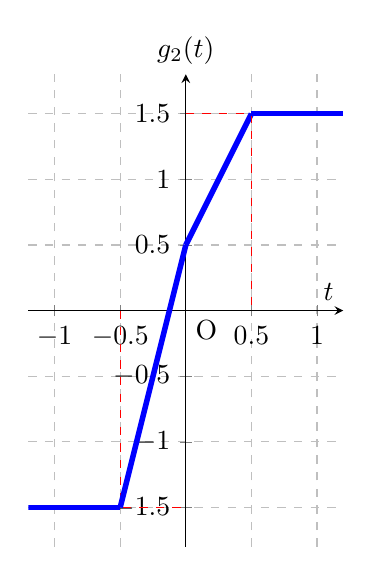
\begin{tikzpicture}
                    \begin{axis}[
                        axis lines = middle,
                        xlabel = {$t$},
                        ylabel = {$g_2(t)$},
                        ylabel style={at={(rel axis cs:0.5, 1)}, anchor=south},
                        xmin = -1.2, xmax = 1.2,
                        ymin = -1.7, ymax = 1.7,
                        xtick distance = 0.5,
                        ytick distance = 0.5,
                        grid = major,
                        grid style = dashed,
                        scale only axis,
                        width = 4cm,
                        height = 6cm,
                        axis equal,
                    ]
                    \addplot[domain=-1.2:-0.5, samples=100, smooth, line width=2pt, blue] {-1.5};
                    \addplot[dashed, red] coordinates {(-0.5, 0) (-0.5, -1.5) (0, -1.5)};
                    \addplot[domain=-0.5:0, samples=100, smooth, line width=2pt, blue] {4 * x + 0.5};
                    \addplot[domain=0:0.5, samples=100, smooth, line width=2pt, blue] {2 * x + 0.5};
                    \addplot[dashed, red] coordinates {(0, 1.5) (0.5, 1.5) (0.5, 0)};
                    \addplot[domain=0.5:1.2, samples=100, smooth, line width=2pt, blue] {1.5};
                    \node at (axis cs:0, 0) [anchor=north west] {O};
                    \end{axis}
                \end{tikzpicture}
                \caption{习题 \theexercise (2) 波形}
                \label{fig:chap1-exercise5-solution2}
            \end{figure}
    \end{enumerate}
\end{solution}

\begin{exercise}
    根据如图 \ref{fig:chap1-exercise6} 所示信号 $f(t)$ 作答,其中 $t \in \set{R}$。
    \begin{enumerate}[label=(\arabic*)]
        \item 绘出 $g_1(t) = f(3t) + f(t) * \delta(t - 2)$ 的波形。
        \item 绘出 $g_2(t) = f(2t) * f(-t)$ 的波形。
    \end{enumerate}

    \begin{figure}[H]
        \centering
        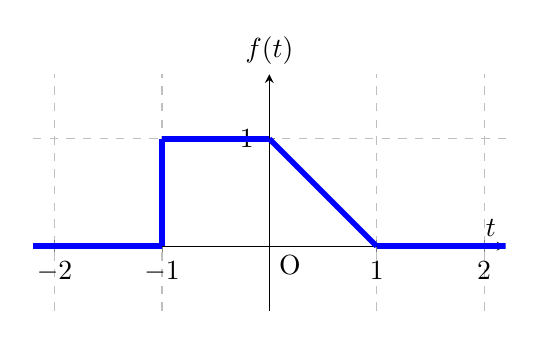
\begin{tikzpicture}
            \begin{axis}[
                axis lines = middle,
                xlabel = {$t$},
                ylabel = {$f(t)$},
                ylabel style={at={(rel axis cs:0.5, 1)}, anchor=south},
                xmin = -2.2, xmax = 2.2,
                ymin = -0.2, ymax = 1.2,
                xtick distance = 1,
                ytick distance = 1,
                grid = major,
                grid style = dashed,
                scale only axis,
                width = 6cm,
                height = 3cm,
                axis equal,
            ]
            \addplot[domain=-2.2:-1, samples=100, smooth, line width=2pt, blue] {0};
            \addplot[smooth, line width=2pt, blue] coordinates {(-1, 0) (-1, 1)};
            \addplot[domain=-1:0, samples=100, smooth, line width=2pt, blue] {1};
            \addplot[domain=0:1, samples=100, smooth, line width=2pt, blue] {1 - x};
            \addplot[domain=1:2.2, samples=100, smooth, line width=2pt, blue] {0};
            \node at (axis cs:0, 0) [anchor=north west] {O};
            \end{axis}
        \end{tikzpicture}
        \caption{习题 \theexercise}
        \label{fig:chap1-exercise6}
    \end{figure}
\end{exercise}

\begin{solution}
    \begin{enumerate}[label=(\arabic*)]
        \item 由题意可得
            \begin{align*}
                g_1(t) & = f(3t) + f(t) * \delta(t - 2) \\
                & = f(3t) + f(t - 2).
            \end{align*}

            因此,$g_1(t)$ 可以看作是 $f(t)$ 沿 $t$ 轴左右平移 $2$ 格后,叠加 $f(3t)$ 的波形。
            绘制波形如图 \ref{fig:chap1-exercise6-solution1} 所示。
            \begin{figure}[H]
                \centering
                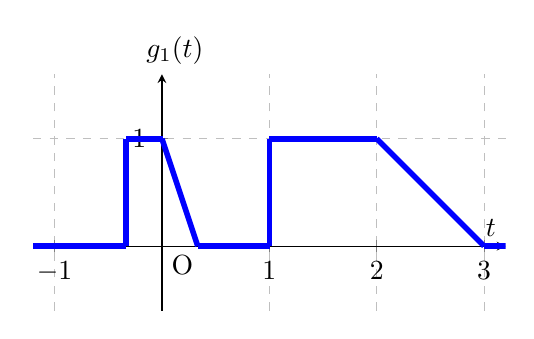
\begin{tikzpicture}
                    \begin{axis}[
                        axis lines = middle,
                        xlabel = {$t$},
                        ylabel = {$g_1(t)$},
                        ylabel style={at={(rel axis cs:0.3, 1)}, anchor=south},
                        xmin = -1.2, xmax = 3.2,
                        ymin = -0.2, ymax = 1.2,
                        xtick distance = 1,
                        ytick distance = 1,
                        grid = major,
                        grid style = dashed,
                        scale only axis,
                        width = 6cm,
                        height = 3cm,
                        axis equal,
                    ]
                    \addplot[domain=-1.2:-1/3, samples=100, smooth, line width=2pt, blue] {0};
                    \addplot[smooth, line width=2pt, blue] coordinates {(-1/3, 0) (-1/3, 1)};
                    \addplot[domain=-1/3:0, samples=100, smooth, line width=2pt, blue] {1};
                    \addplot[domain=0:1/3, samples=100, smooth, line width=2pt, blue] {1 - 3 * x};
                    \addplot[domain=1/3:1, samples=100, smooth, line width=2pt, blue] {0};
                    \addplot[smooth, line width=2pt, blue] coordinates {(1, 0) (1, 1)};
                    \addplot[domain=1:2, samples=100, smooth, line width=2pt, blue] {1};
                    \addplot[domain=2:3, samples=100, smooth, line width=2pt, blue] {3 - x};
                    \addplot[domain=3:3.2, samples=100, smooth, line width=2pt, blue] {0};
                    \node at (axis cs:0, 0) [anchor=north west] {O};
                    \end{axis}
                \end{tikzpicture}
                \caption{习题 \theexercise (1) 波形}
                \label{fig:chap1-exercise6-solution1}
            \end{figure}
        \item 由题意可得
            \begin{align*}
                g_2(t) & = f(2t) * f(-t) \\
                & = \int_{-\infty}^{+\infty}f(2a)f(a - t)\D{a} \\
                & = \int_{t - 1}^{t}f(2a)\D{a} + \int_{t}^{t + 1}(1 + t - a)f(2a)\D{a}.
            \end{align*}

            \begin{enumerate}
                \item 当 $t \le -\frac{3}{2}$ 时,有
                    \begin{align*}
                        g_2(t) & = \int_{t - 1}^{t}0\;\D{a} + \int_{t}^{t + 1}(1 + t - a)\cdot 0\;\D{a} \\
                        & = 0.
                    \end{align*}
                \item 当 $-\frac{3}{2} < t \le -1$ 时,有
                    \begin{align*}
                        g_2(t) & = \int_{t - 1}^{t}0\;\D{a} + \int_{t}^{-1/2}(1 + t - a)\cdot 0\;\D{a} + \int_{-1/2}^{t + 1}(1 + t - a)\cdot 1\;\D{a} \\
                        & = 0 + 0 + \left.\left(-\frac{1}{2}a^2 + (t + 1)a\right)\right|_{a = -1/2}^{a = t + 1} \\
                        & = \frac{1}{2}(t + 1)^2 - \left(-\frac{1}{8} - \frac{t + 1}{2}\right) \\
                        & = \frac{1}{2}t^2 + \frac{3}{2}t + \frac{9}{8}.
                    \end{align*}
                \item 当 $-1 < t \le -\frac{1}{2}$ 时,有
                    \begin{align*}
                        g_2(t) & = \int_{t - 1}^{t}0\;\D{a} + \int_{t}^{-1/2}(1 + t - a)\cdot 0\;\D{a} + \int_{-1/2}^{0}(1 + t - a) \cdot 1\;\D{a} + \int_{0}^{t + 1}(1 + t - a)(1 - 2a)\D{a} \\
                        & = \int_{t - 1}^{t}0\;\D{a} + \int_{t}^{-1/2}0\;\D{a} + \int_{-1/2}^{0}(1 + t - a)\D{a} + \int_{0}^{t + 1}(2a^2 - (2t + 3)a + t + 1)\D{a} \\
                        & = 0 + 0 + \left.\left(-\frac{1}{2}a^2 + (t + 1)a\right)\right|_{a = -1/2}^{a = 0} + \left.\left(\frac{2}{3}a^3 - \frac{2t + 3}{2}a^2 + (t + 1)a\right)\right|_{a = 0}^{a = t + 1} \\
                        & = 0 - \left(-\frac{1}{8} - \frac{t + 1}{2}\right) + \left(\frac{2}{3}(t + 1)^3 - \frac{2t + 3}{2}(t + 1)^2 + (t + 1)^2\right) \\
                        & = -\frac{1}{3}t^3 - \frac{1}{2}t^2 + \frac{1}{2}t + \frac{19}{24}.
                    \end{align*}
                \item 当 $-\frac{1}{2} < t \le 0$ 时,
                    \begin{align*}
                        g_2(t) & = \int_{t - 1}^{-1/2}0\;\D{a} + \int_{-1/2}^{t}1\;\D{a} + \int_{t}^{0}(1 + t - a)\cdot 1\;\D{a} + \int_{0}^{1/2}(1 + t - a)(1 - 2a)\D{a} + \int_{1/2}^{t + 1}(1 + t - a)\cdot 0\;\D{a} \\
                        & = 0 + t + \frac{1}{2} + \left.\left(-\frac{1}{2}a^2 + (t + 1)a\right)\right|_{a = t}^{a = 0} + \left.\left(\frac{2}{3}a^3 - \frac{2t + 3}{2}a^2 + (t + 1)a\right)\right|_{a = 0}^{a = 1/2} + 0 \\
                        & = t + \frac{1}{2} + 0 - \left(\frac{1}{2}t^2 + t\right) + \left(\frac{1}{4}t - \frac{1}{24}\right) \\
                        & = -\frac{1}{2}t^2 + \frac{1}{4}t + \frac{17}{24}.
                    \end{align*}
                \item 当 $0 < t \le \frac{1}{2}$ 时,有
                    \begin{align*}
                        g_2(t) & = \int_{t - 1}^{-1/2}0\;\D{a} + \int_{-1/2}^{0}1\;\D{a} + \int_{0}^{t}(1 - 2a)\D{a} + \int_{t}^{1/2}(1 + t - a)(1 - 2a)\D{a} + \int_{1/2}^{t + 1}(1 + t - a)\cdot 0\;\D{a} \\
                        & = 0 + \left.\frac{1}{2} + \left(a - a^2\right)\right|_{a = 0}^{a = t} + \left.\left(\frac{2}{3}a^3 - \frac{2t + 3}{2}a^2 + (t + 1)a\right)\right|_{a = t}^{a = 1/2} + 0 \\
                        & = \frac{1}{2} + t - t^2 + \left(\frac{1}{12} - \frac{2t + 3}{8} + \frac{t + 1}{2}\right) - \left(\frac{2}{3}t^3 - (2t + 3){2}t^2 + t(t + 1)\right) \\
                        & = \frac{1}{3}t^3 - \frac{1}{2}t^2 + \frac{1}{4}t + \frac{17}{24}.
                    \end{align*}
                \item 当 $\frac{1}{2} < t \le 1$ 时,有
                    \begin{align*}
                        g_2(t) & = \int_{t - 1}^{0}1\;\D{a} + \int_{0}^{1/2}(1 - 2a)\D{a} + \int_{1/2}^{t}0\;\D{a} + \int_{t}^{t + 1}(1 + t - a)\cdot 0\;\D{a} \\
                        & = 1 - t + \left.\left(-a^2 + a\right)\right|_{a = 0}^{a = 1/2} + 0 + 0 \\
                        & = 1 - t + \frac{1}{4} \\
                        & = -t + \frac{5}{4}.
                    \end{align*}
                \item 当 $1 < t \le \frac{3}{2}$ 时,有
                    \begin{align*}
                        g_2(t) & = \int_{t - 1}^{1/2}(1 - 2a)\D{a} + \int_{1/2}^{t}0\;\D{a} + \int_{t}^{t + 1}(1 + t - a)\cdot 0\;\D{a} \\
                        & = \left.\left(-a^2 + a\right)\right|_{a = t - 1}^{a = 1/2} + 0 + 0 \\
                        & = \frac{1}{4} - (-(t - 1)^2 + (t - 1)) \\
                        & = t^2 - 3t + \frac{9}{4}.
                    \end{align*}
                \item 当 $t > \frac{3}{2}$ 时,有
                    \begin{align*}
                        g_2(t) & = \int_{t - 1}^{t}0\;\D{a} + \int_{t}^{+\infty}(1 + t - a)\cdot 0\;\D{a} \\
                        & = 0.
                    \end{align*}
            \end{enumerate}

            因此,$g_2(t)$ 的表达式为
            \begin{align*}
                g_2(t) = \begin{cases}
                    0, & t \le -\frac{3}{2}, \\
                    \frac{1}{2}t^2 + \frac{3}{2}t + \frac{9}{8}, & -\frac{3}{2} < t \le -1, \\
                    -\frac{1}{3}t^3 - \frac{1}{2}t^2 + \frac{1}{2}t + \frac{19}{24}, & -1 < t \le -\frac{1}{2}, \\
                    -\frac{1}{2}t^2 + \frac{1}{4}t + \frac{17}{24}, & -\frac{1}{2} < t \le 0, \\
                    \frac{1}{3}t^3 - \frac{1}{2}t^2 + \frac{1}{4}t + \frac{17}{24}, & 0 < t \le \frac{1}{2}, \\
                    -t + \frac{5}{4}, & \frac{1}{2} < t \le 1, \\
                    t^2 - 3t + \frac{9}{4}, & 1 < t \le \frac{3}{2}, \\
                    0, & t > \frac{3}{2}.
                \end{cases}
            \end{align*}

            绘制波形如图 \ref{fig:chap1-exercise6-solution2} 所示。
            \begin{figure}[H]
                \centering
                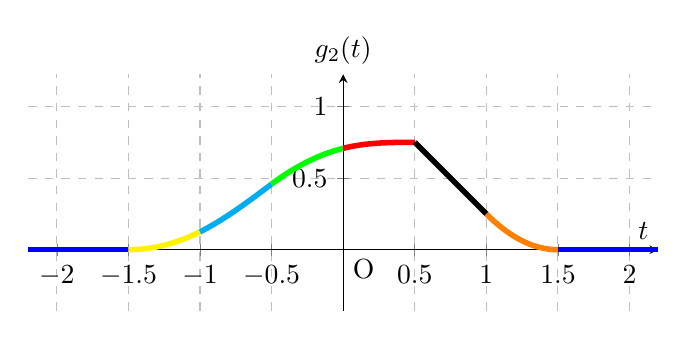
\begin{tikzpicture}
                    \begin{axis}[
                        axis lines = middle,
                        xlabel = {$t$},
                        ylabel = {$g_2(t)$},
                        ylabel style={at={(rel axis cs:0.5, 1)}, anchor=south},
                        xmin = -2.2, xmax = 2.2,
                        ymin = -0.2, ymax = 1,
                        xtick distance = 0.5,
                        ytick distance = 0.5,
                        grid = major,
                        grid style = dashed,
                        scale only axis,
                        width = 8cm,
                        height = 3cm,
                        axis equal,
                    ]
                    \addplot[domain=-2.2:-1.5, samples=100, smooth, line width=2pt, blue] {0};
                    \addplot[domain=-1.5:-1, samples=100, smooth, line width=2pt, yellow] {0.5 * x^2 + 1.5 * x + 9/8};
                    \addplot[domain=-1:-0.5, samples=100, smooth, line width=2pt, cyan] {-1/3 * x^3 - 1/2 * x^2 + 1/2 * x + 19/24};
                    \addplot[domain=-0.5:0, samples=100, smooth, line width=2pt, green] {-1/2 * x^2 + 1/4 * x + 17/24};
                    \addplot[domain=0:0.5, samples=100, smooth, line width=2pt, red] {1/3 * x^3 - 1/2 * x^2 + 1/4 * x + 17/24};
                    \addplot[domain=0.5:1, samples=100, smooth, line width=2pt, black] {-x + 5/4};
                    \addplot[domain=1:1.5, samples=100, smooth, line width=2pt, orange] {x^2 - 3 * x + 9/4};
                    \addplot[domain=1.5:2.2, samples=100, smooth, line width=2pt, blue] {0};
                    \node at (axis cs:0, 0) [anchor=north west] {O};
                    \end{axis}
                \end{tikzpicture}
                \caption{习题 \theexercise (2) 波形}
                \label{fig:chap1-exercise6-solution2}
            \end{figure}
    \end{enumerate}
\end{solution}
